\section{Structural Retrieval Methodology}
\label{sec:methodology}

The core retrieval task translates a natural-language description into a ranked list of code entities. CodeGraph splits this into two steps: selecting lexical seeds, and propagating relevance through the graph.

\subsection{Seed Selection}

Personalized PageRank requires a set of starting points in the graph. Seed selection provides these starting points by translating the natural-language task description into a personalization vector: a probability distribution over graph nodes that determines where restart mass is placed during the random walk.

CodeGraph constructs this personalization vector from three complementary signals:
\begin{enumerate}
    \item \textbf{Entity match (weight 0.6):} Extracts direct identifier mentions (CamelCase, snake\_case, backtick-quoted names) from the task text using regex patterns and matches them against the graph's node vocabulary. Highly ambiguous names are down-weighted using inverse-document-frequency scaling to prevent common words like \texttt{update} from dominating the distribution.
    \item \textbf{BM25 keyword search (weight 0.3):} Broadens coverage when explicit identifiers are absent. Each graph entity is indexed as a document built from its short name, qualified name, path tokens, and the first 200 characters of its docstring. Crucially, a compound tokenization step splits names at CamelCase boundaries and underscores. This ensures that abstract queries (e.g., ``SQL compilation'') can match composite identifiers (e.g., \texttt{SQLCompiler}) that would otherwise remain invisible to standard tokenization.
    \item \textbf{Issue path hint (weight 0.2):} Extracts directory fragments or file names mentioned in the issue text and maps them to file nodes or entities located under the corresponding path. This accommodates developers who frequently cite file paths rather than function names when reporting bugs.
\end{enumerate}

These three signals are merged and normalized into a single personalization vector, forming a robust starting distribution that does not rely exclusively on perfect entity resolution. CodeGraph assigns each matched seed an initial confidence score based on the signals above, but notably does not use these scores to weight the PPR restart probabilities (as discussed in \Cref{sec:evaluation}).

\subsection{IDF-Based Edge Reweighting}

Uniform base weights assume that every structural connection contributes equally to retrieval, but this is not true in practice. Some targets are highly specific, while others are generic utility nodes (e.g., global loggers, base classes) reused across large parts of the repository. If both receive the same edge weight, Personalized PageRank sends too much probability into broadly shared utility neighborhoods, weakening the ranking of domain-specific code.

To account for this effect, CodeGraph assigns each edge a weight based on the in-degree of its target node:
\begin{equation}
    w(e) = \frac{1}{\log_2\!\bigl(\operatorname{in\_degree}(v) + 2\bigr)}
    \label{eq:idf-weight}
\end{equation}
Nodes with many incoming edges receive lower weights, while rare or specialized targets retain stronger weights. This logarithmic penalty reduces hub influence gradually. \Cref{fig:idf-reweighting} illustrates the intuition: instead of splitting relevance equally, probability is steered away from ubiquitous hubs.

\begin{figure}[htbp]
    \centering
    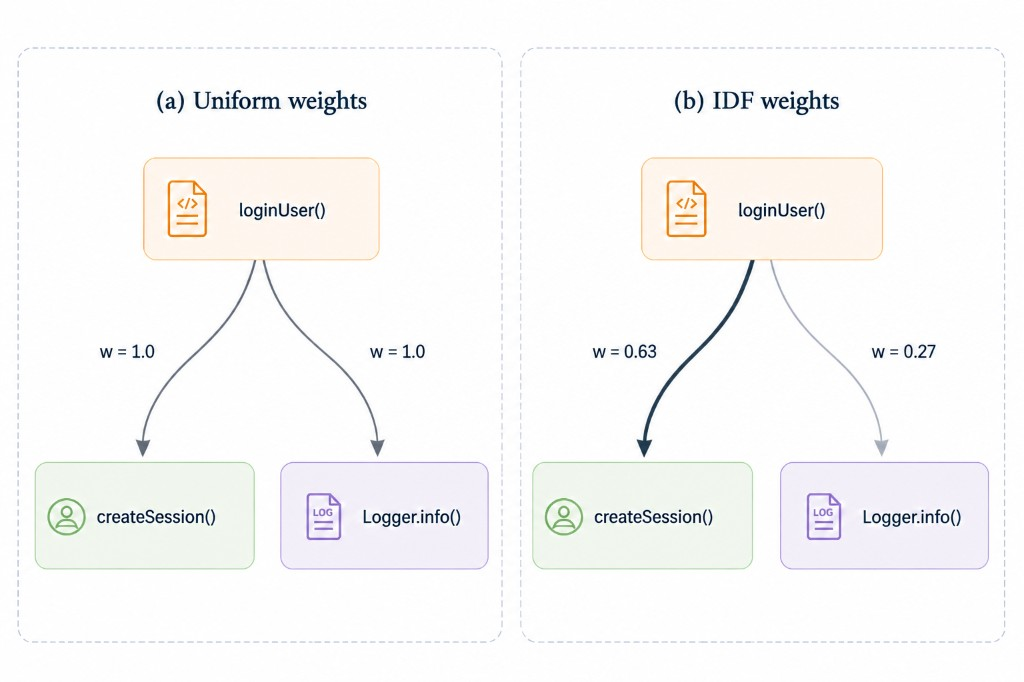
\includegraphics[width=\linewidth]{assets/idf_reweighting.png}
    \caption{IDF edge reweighting (same seed, two outgoing edges). Panel (a) keeps uniform weights; Panel (b) lowers the weight toward the high in-degree hub so more relevance mass stays on the domain-specific callee.}
    \label{fig:idf-reweighting}
\end{figure}

\subsection{Personalized PageRank Configuration}

CodeGraph utilizes the Neo4j Graph Data Science (GDS) library, projecting the graph into memory as undirected edges to allow relevance to flow both downstream (callees) and upstream (callers). 

Two critical design choices govern the PPR execution:
\begin{itemize}
    \item \textbf{Uniform Restart Mode:} Instead of giving highly-weighted seeds more restart probability, CodeGraph uses a uniform distribution across all selected seeds. Weighting by confidence amplifies ambiguous lexical matches (false positives). Uniform restart provides every seed an equal chance, allowing the graph topology itself to arbitrate: correct seeds that share structural paths compound their PPR mass, while isolated incorrect seeds dissipate.
    \item \textbf{Damping Factor ($d=0.70$):} A lower damping factor keeps the random walk closer to the seed nodes on each step. This improves early-rank precision and reduces the expected random walk length, allowing PPR to converge in 6--10 iterations.
\end{itemize}

\subsection{Context Delivery and MCP Integration}

The ranked list produced by PPR must be packaged for the AI agent. Post-processing deduplicates entities from the same file, extracts the specific source code spans from the file system, and enforces a strict token budget (default 6,000 tokens) to ensure it fits within the agent's context window. If multiple sub-entities from the same file are highly ranked, CodeGraph drops the parent \texttt{File} node to avoid wasting the token budget on the entire file's content, retaining only the relevant sub-entity snippets.

CodeGraph wraps this entire retrieval pipeline into a Model Context Protocol (MCP) server. The server exposes a \texttt{get\_relevant\_context} tool, enabling AI agents to programmatically fetch ranked source snippets by providing only the task description. When explanation mode is enabled, the system attaches a seed provenance trace and a short structural reasoning path to each result. This trace identifies which seeds triggered the result and through which graph edges the relevance propagated, providing an essential trust signal for the agent.
